% FedFlow-LLM final presentation (23AID206 Introduction to Computer Networks)
% Build:  cd slides && latexmk -pdf main.tex
% Every number is checked against a repo file; the \note of each frame names the file.
\documentclass[11pt,aspectratio=169]{beamer}

\usetheme{Madrid}                       % stock theme: footline carries the slide number
\setbeamertemplate{navigation symbols}{}% hide the navigation icons
\usepackage[T1]{fontenc}                % so \detokenize'd paths print underscores
\usepackage{booktabs}
\usepackage{array}
\usepackage{tikz}
\usetikzlibrary{positioning,arrows.meta,shapes.geometric}

% ---------- one colour per routing mode, used in every table and diagram ----------
\definecolor{cStatic}{RGB}{110,110,110}
\definecolor{cReactive}{RGB}{217,95,2}
\definecolor{cModel}{RGB}{31,119,180}
\definecolor{cOracle}{RGB}{27,140,60}
\definecolor{cAlt}{RGB}{128,80,170}
\newcommand{\mStatic}{\textcolor{cStatic}{\textbf{static}}}
\newcommand{\mReactive}{\textcolor{cReactive}{\textbf{reactive}}}
\newcommand{\mModel}{\textcolor{cModel}{\textbf{model}}}
\newcommand{\mOracle}{\textcolor{cOracle}{\textbf{oracle}}}
\newcommand{\mAlt}{\textcolor{cAlt}{\textbf{alt}}}

% Source-file names in notes; \detokenize keeps underscores literal.
\newcommand{\src}[1]{\texttt{\detokenize{#1}}}

% Figure from the figure step, or a visible placeholder if it does not exist yet.
% #1 = figure name (no extension), #2 = width, #3 = height
\newcommand{\fedfig}[3]{%
  \IfFileExists{../figures/#1.pdf}{\includegraphics[width=#2,height=#3,keepaspectratio]{../figures/#1.pdf}}{%
  \IfFileExists{../figures/#1.png}{\includegraphics[width=#2,height=#3,keepaspectratio]{../figures/#1.png}}{%
  \fbox{\parbox[c][#3][c]{\dimexpr#2-2\fboxsep-2\fboxrule\relax}{\centering\color{red}\footnotesize\textbf{figure not yet generated:}\\\texttt{\detokenize{#1}}}}}}}

% Small boxed line for claims that must stay with their figure.
\newcommand{\claim}[1]{\colorbox{yellow!20}{\parbox{\dimexpr\linewidth-2\fboxsep\relax}{\footnotesize #1}}}

\title[FedFlow-LLM]{FedFlow-LLM}
\subtitle{Does forecast-driven rerouting give lower delay than reactive rerouting in an emulated SDN?}
\author[{[TEAM MEMBER NAMES]}]{[TEAM MEMBER NAMES]\\[2pt]{\small [ROLL NUMBERS]}}
\institute[Amrita]{[COURSE] 23AID206 Introduction to Computer Networks\\
  [INSTRUCTOR] Dr.\ Sundaresan S\\
  [INSTITUTION] Amrita School of Artificial Intelligence, Amrita Vishwa Vidyapeetham, Coimbatore}
\date{}

\begin{document}

% ================= 1 Title =================
\begin{frame}
  \titlepage
  \note{Time 0:30. ``We are presenting FedFlow-LLM, a course project in computer networks. One question: does forecast-driven rerouting give lower delay than reactive rerouting in an emulated software-defined network?'' No numbers on this slide.}
\end{frame}

% ================= 2 Problem statement =================
\begin{frame}{Problem statement}
  \begin{itemize}
    \item Reactive rerouting acts only after load rises
    \item Congestion on the primary link raises delay
    \item A forecast could move traffic earlier
    \item Traffic data stays at each cell (privacy)
    \item Question: is forecast-driven delay lower than reactive?
  \end{itemize}
  \note{Time 1:00. ``A reactive controller only sees load after it has arrived. If the primary link is already full, packets queue and delay rises. A forecast could, in principle, move traffic before the jump. Traffic records are per cell and sensitive, so we train with federated learning instead of pooling the data.'' No numbers on this slide.}
\end{frame}

% ================= 3 Objectives =================
\begin{frame}{Objectives}
  \begin{enumerate}
    \item Train a federated LoRA traffic forecaster
    \item Feed its forecast to an SDN controller
    \item Compare five routing modes on delay
    \item Compare forecast error with simple baselines
    \item State plainly what the results do not show
  \end{enumerate}
  \note{Time 1:00. ``Five objectives. Train a small language model as a traffic forecaster with federated LoRA. Connect its forecast to a POX controller that picks a path. Compare five routing modes on delay, loss and route flips. Check forecast error against repeat-last and moving-average baselines. And list the limits.'' No numbers on this slide besides the count of modes (five, from \src{experiments/run_experiment.py} MODES).}
\end{frame}

% ================= 4-6 Literature review =================
\newcommand{\litcols}{\setlength\tabcolsep{3pt}\renewcommand{\arraystretch}{1.15}%
  \begin{tabular}{@{}>{\raggedright}p{0.5cm}>{\raggedright}p{2.9cm}>{\raggedright}p{3.4cm}>{\raggedright}p{3.4cm}>{\raggedright\arraybackslash}p{2.9cm}@{}}}
\newcommand{\lithead}{\toprule \textbf{S.No} & \textbf{Journal/Conference name, Publisher, Year} & \textbf{Technique adopted} & \textbf{Inference} & \textbf{Cons}\tabularnewline \midrule}

\begin{frame}{Literature review (1/3): routing and SDN with federated learning}
  \footnotesize
  \litcols \lithead
  1 & IEEE Internet of Things Journal, IEEE, 2026 \cite{yang2026hfrl} & GCN-LSTM-Attention utilisation forecast + hierarchical federated RL routing & Forecast-aware routing kept lower steady-state end-to-end latency than DDQN, SP and ELB & Starlink simulation only; satellite topology, not SDN emulation\tabularnewline\midrule
  2 & IEEE Access, IEEE, 2026 \cite{silva2026netlink} & NetLinkClassifier: federated model classifies link utilisation from traffic matrices at an SDN edge layer & Link load estimated without per-link sensors; used by a routing VNF & Classifies current link state; no forecast of future load\tabularnewline\midrule
  3 & The Journal of Supercomputing, Springer, 2026 \cite{sadeghi2026sdmart} & SDMART: attention-based deep federated learning for cache replacement in distributed SDN with NDN & Federated learning used inside SDN control decisions & Caching task, not routing or delay\tabularnewline
  \bottomrule\end{tabular}
  \note{Time 0:45. ``Three works from 2026 that put federated learning near routing or SDN control.''
  Records: [1] Crossref DOI 10.1109/JIOT.2026.3708793 (IEEE IoT J vol 13 no 18, 2026); abstract read from Semantic Scholar record of that DOI. [2] Crossref DOI 10.1109/ACCESS.2026.3675110 (IEEE Access vol 14, 2026); abstract from OpenAlex record of that DOI. [3] Crossref DOI 10.1007/s11227-026-08655-7 (J. Supercomputing vol 82, 2026); full abstract not readable (publisher login); technique taken from the Semantic Scholar summary of that DOI. Cons column = scope difference from our question, read from the abstract.}
\end{frame}

\begin{frame}{Literature review (2/3): cellular traffic forecasting}
  \footnotesize
  \litcols \lithead
  4 & IEEE Access, IEEE, 2026 \cite{yuliana2026hybrid} & Hybrid LSTM-Transformer with time embedding; KPI data from 23 cells, Bandung, four months & Reports $R^2=0.9357$, RMSE $=0.9822$; lower error than ARIMA, LSTM, ConvLSTM & Centralised training; forecasting only, no routing action\tabularnewline\midrule
  5 & IEEE Transactions on Mobile Computing, IEEE, 2026 \cite{wang2026mobilellm} & MobileLLM: partially frozen GPT-2 fuses traffic tokens with semantic context & MAE gains of 0.88\% to 32.62\% over baselines on Milan, Trentino, Shanghai & Centralised; no network control loop\tabularnewline\midrule
  6 & IEEE Transactions on Intelligent Transportation Systems, IEEE, 2025 \cite{rong2025stgllm} & STGLLM-E: spatio-temporal generative LLM, trained on edge servers over road subgraphs & Better accuracy and training efficiency than baselines on two road datasets & Road traffic, not network traffic; no routing\tabularnewline
  \bottomrule\end{tabular}
  \note{Time 0:45. ``Forecasting work. Note row 5 uses the same Milan data source as we do.''
  Records: [4] Crossref DOI 10.1109/ACCESS.2026.3669215; R2 0.9357 and RMSE 0.9822 are from its abstract (OpenAlex record). [5] Crossref DOI 10.1109/TMC.2026.3684577 (IEEE TMC vol 25 no 9, 2026); 0.88\% to 32.62\% from its abstract (OpenAlex). [6] Crossref DOI 10.1109/TITS.2024.3456890 (IEEE T-ITS vol 26 no 10, issue Oct 2025; online 17 Sep 2024 per OpenAlex). These numbers are theirs, not ours.}
\end{frame}

\begin{frame}{Literature review (3/3): LLMs for telecom decisions}
  \footnotesize
  \litcols \lithead
  7 & IEEE Communications Surveys \& Tutorials, IEEE, 2025 \cite{zhou2025llmtelecom} & Survey: LLMs for generation, classification, optimisation and prediction in telecom & Names time-series traffic prediction as an LLM telecom task & Survey; no new measurements\tabularnewline\midrule
  8 & IEEE Communications Surveys \& Tutorials, IEEE, 2026 \cite{yang2026dmllm} & Survey: prompt learning, chain of thought, decision frameworks, multi-agent LLMs & LLM use for wireless decisions is ``fragmented and exploratory'' & Survey; no emulated network results\tabularnewline
  \bottomrule\end{tabular}
  \vspace{4pt}
  {\footnotesize Only works from 2021--2026 with a checked DOI record are listed.}
  \note{Time 0:45. ``Two surveys that place LLM forecasting and decision making in telecom.''
  Records: [7] Crossref DOI 10.1109/COMST.2024.3465447 (IEEE COMST vol 27 no 3, issue June 2025; online 23 Sep 2024). [8] Crossref DOI 10.1109/COMST.2025.3614494 (IEEE COMST vol 28, 2026; online 25 Sep 2025). Quoted phrase is from the [8] abstract (OpenAlex). Two 2026 works from the brief (National Academy Science Letters; Simulation Modelling Practice and Theory) are in the references but not this table: their abstracts were not readable, see SLIDES\_DECISIONS.md.}
\end{frame}

% ================= 7 Research gap and novelty =================
\begin{frame}{Research gap and novelty}
  \begin{itemize}
    \item Forecasting papers stop at forecast error
    \item Routing papers use simulators, not SDN emulation
    \item Few test a small LLM forecaster in the loop
    \item \textbf{Our novelty: the combination}
    \item Federated small-LLM forecast $\rightarrow$ SDN reroute, emulated network
  \end{itemize}
  \note{Time 1:00. ``The forecasting papers we read report forecast error and stop. The routing papers use simulators. What we add is the combination: a federated, LoRA-tuned small LLM whose forecast drives an SDN reroute decision, tested in an emulated network with a real controller. We do not claim it is the first of its kind.'' No numbers on this slide.}
\end{frame}

% ================= 8 Methodology: system overview =================
\begin{frame}{Methodology (1/5): system overview}
  \centering
  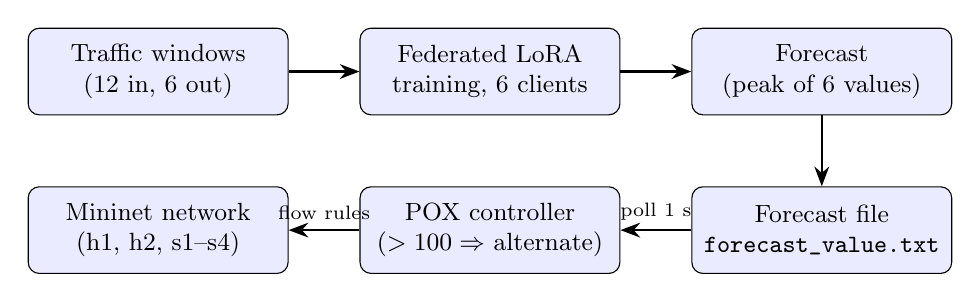
\begin{tikzpicture}[
      box/.style={draw, rounded corners, fill=blue!8, align=center, minimum width=3.3cm, minimum height=1.1cm, font=\small},
      arr/.style={-{Stealth[length=2.5mm]}, thick}, node distance=0.9cm and 0.9cm]
    \node[box] (tw) {Traffic windows\\(12 in, 6 out)};
    \node[box, right=of tw] (fl) {Federated LoRA\\training, 6 clients};
    \node[box, right=of fl] (fc) {Forecast\\(peak of 6 values)};
    \node[box, below=of fc] (file) {Forecast file\\\texttt{\detokenize{forecast_value.txt}}};
    \node[box, left=of file] (pox) {POX controller\\($>100 \Rightarrow$ alternate)};
    \node[box, left=of pox] (mn) {Mininet network\\(h1, h2, s1--s4)};
    \draw[arr] (tw) -- (fl);
    \draw[arr] (fl) -- (fc);
    \draw[arr] (fc) -- (file);
    \draw[arr] (file) -- node[above, font=\scriptsize]{poll 1 s} (pox);
    \draw[arr] (pox) -- node[above, font=\scriptsize]{flow rules} (mn);
  \end{tikzpicture}
  \note{Time 1:30. ``Left to right: traffic windows train a federated LoRA model with six clients. At run time the model's forecast becomes one number, the peak of its six predicted values. That number goes into a file. The POX controller reads the file every second; above 100 it sends traffic on the alternate path. Mininet carries the traffic.''
  Sources: 12 in / 6 out from the prompt in \src{training/data/telecom/traffic_train.json}; 6 clients in \src{training/client.py} (NUM\_CLIENTS); poll 1 s and threshold 100 in \src{controller/reroute_trigger.py} (CHECK\_INTERVAL, THRESHOLD); peak of 6 in \src{experiments/run_experiment.py} (mode docstring).}
\end{frame}

% ================= 9 Methodology: data and windows =================
\begin{frame}{Methodology (2/5): data and windows}
  \begin{columns}[T]
    \column{0.52\textwidth}
    \begin{itemize}
      \item Telecom Italia, Milan, Nov 2013 \cite{barlacchi2015milan,telecomitalia2015dataverse}
      \item Six grid cells; tested: 7511, 8336
      \item 12 past values in, next 6 out
      \item Scaled so 100 = 10 Mbps
      \item Also one synthetic traffic series
    \end{itemize}
    \column{0.45\textwidth}
    \footnotesize
    \begin{tabular}{@{}ll@{}}
      \toprule
      Slot length & 10 min \\
      Days used & 1--14 Nov 2013 \\
      Train / val / test & slots 0--1439 / 1440--1727 / 1728--2015\\
      Test windows & 366 (telecom), 91 (synthetic)\\
      Output text & \texttt{PREDICTION: v1, \ldots, v6}\\
      \bottomrule
    \end{tabular}
  \end{columns}
  \note{Time 1:00. ``Internet activity from the Milan grid, November 2013. Six cells, one per client; the network test used cells 7511 and 8336. Each example gives 12 past values and asks for the next 6. One scale factor maps the data so that 100 means the 10 Mbps primary link.''
  Sources: dates, cells, split, 10-min slots, scale rule in \src{datasets/telecom_milan/README.md}; 366 windows in \src{results/final_telecom/outputs/metrics.json} (windows\_used); 91 in \src{results/final/SUMMARY.md}; prompt format in \src{training/data/telecom/traffic_train.json}. DOI 10.7910/DVN/EGZHFV (DataCite record) and 10.1038/sdata.2015.55 (Crossref).}
\end{frame}

% ================= 10 Methodology: federated LoRA =================
\begin{frame}{Methodology (3/5): federated LoRA training}
  \begin{columns}[T]
    \column{0.5\textwidth}
    \begin{itemize}
      \item FedAvg over 6 clients \cite{mcmahan2017fedavg,beutel2020flower}
      \item Telecom: client $i$ trains on cell $i$
      \item 25 rounds, 200 training examples
      \item Base model frozen; only LoRA shared \cite{hu2021lora}
    \end{itemize}
    \column{0.46\textwidth}
    \footnotesize
    \begin{tabular}{@{}ll@{}}
      \toprule
      Base model & Qwen2.5-1.5B-Instruct \cite{qwen2024qwen25}\\
      LoRA rank / alpha & 8 / 16\\
      Target modules & \texttt{q\_proj}, \texttt{v\_proj}\\
      LoRA dropout & 0.05\\
      Optimiser & AdamW, lr $10^{-4}$\\
      \bottomrule
    \end{tabular}
  \end{columns}
  \note{Time 1:00. ``Flower runs FedAvg over six simulated clients. On the telecom data, client i only sees windows from cell i. Twenty-five rounds, 200 training examples in all. Only the LoRA adapter is trained and averaged.''
  Sources: rank 8, alpha 16, q\_proj/v\_proj, dropout 0.05, lr 1e-4, model name in \src{training/client.py}; 25 rounds and FedAvg in \src{training/server.py} (NUM\_ROUNDS); 200 examples = length of \src{training/data/telecom/traffic_train.json}; client i = cell i because \src{training/data/telecom/train_starts.json} cycles cells 0--5 and \src{training/client.py} takes every 6th example.}
\end{frame}

% ================= 11 Methodology: network and controller =================
\begin{frame}{Methodology (4/5): emulated network and controller}
  \begin{columns}[c]
    \column{0.55\textwidth}
    \centering
    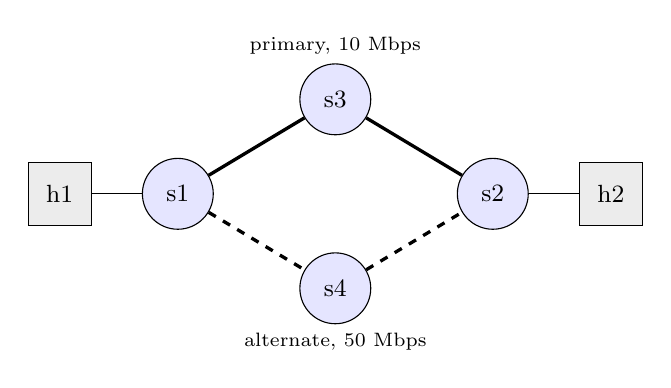
\begin{tikzpicture}[
        sw/.style={draw, circle, fill=blue!10, minimum size=0.9cm, font=\small},
        host/.style={draw, rectangle, fill=gray!15, minimum size=0.8cm, font=\small}]
      \node[host] (h1) at (0,0) {h1};
      \node[sw] (s1) at (1.5,0) {s1};
      \node[sw] (s3) at (3.5,1.2) {s3};
      \node[sw] (s4) at (3.5,-1.2) {s4};
      \node[sw] (s2) at (5.5,0) {s2};
      \node[host] (h2) at (7,0) {h2};
      \draw (h1) -- (s1); \draw (s2) -- (h2);
      \draw[very thick] (s1) -- (s3) -- (s2);
      \draw[very thick, dashed] (s1) -- (s4) -- (s2);
      \node[font=\scriptsize, above] at (3.5,1.65) {primary, 10 Mbps};
      \node[font=\scriptsize, below] at (3.5,-1.65) {alternate, 50 Mbps};
    \end{tikzpicture}
    \column{0.43\textwidth}
    \begin{itemize}\small
      \item Fixed forwarding tables, no flooding
      \item Static ARP on both hosts
      \item File polled every 1 s
      \item Value $>100$: alternate, else primary
    \end{itemize}
  \end{columns}
  \note{Time 1:30. ``Two hosts, four switches. The primary path through s3 is 10 Mbps; the alternate through s4 is 50 Mbps. The topology has a loop, so the controller never floods; it uses fixed tables, and the hosts have static ARP. Every second it reads the forecast file: above 100 means alternate.''
  Sources: topology and link rates in \src{controller/topo.py} and \src{CLAUDE.md}; poll 1 s, threshold 100 and the strict ``$>$'' rule in \src{controller/reroute_trigger.py} (decide\_path). Mininet \cite{lantz2010mininet}, OpenFlow \cite{mckeown2008openflow}.}
\end{frame}

% ================= 12 Methodology: modes, metrics, claim rule =================
\begin{frame}{Methodology (5/5): routing modes, metrics, claim rule}
  \footnotesize
  \begin{columns}[T]
    \column{0.55\textwidth}
    \begin{tabular}{@{}ll@{}}
      \toprule
      Mode & Value written each step\\ \midrule
      \mStatic & 0 (primary always)\\
      \mReactive & true value of previous step\\
      \mModel & peak of model's 6 predictions\\
      \mOracle & peak of 6 true values, same window\\
      \mAlt & 1000 (alternate always; reference)\\
      \bottomrule
    \end{tabular}
    \column{0.42\textwidth}
    \textbf{Metrics}: mean ping delay (ms), UDP loss, route flips, share of steps written above 100.\\[6pt]
    \textbf{Claim rule}: ``lower'' only if every \mModel{} run is below every \mReactive{} run on that cell; otherwise ``no ordering claimed''.
  \end{columns}
  \note{Time 1:00. ``Five modes differ only in the number written to the file each step. Static never leaves the primary path, alt never leaves the alternate, oracle sees the true future, reactive sees the last true value, and model uses the forecast. We say `lower' only if all three model runs sit below all three reactive runs on a cell.''
  Sources: mode definitions in \src{experiments/run_experiment.py} (docstring and build\_steps); metrics are columns of \src{results/experiment_telecom/7511/summary.csv}. The claim rule is the one in the task brief; it is not written in a repo file on main (see SLIDES\_DECISIONS.md).}
\end{frame}

% ================= 13 Implementation: stack =================
\begin{frame}{Implementation (1/5): software stack}
  \centering\small
  \begin{tabular}{@{}lll@{}}
    \toprule
    Layer & Tool & Role\\ \midrule
    Model & Qwen2.5-1.5B-Instruct \cite{qwen2024qwen25} & traffic forecaster\\
    Federated learning & Flower \cite{beutel2020flower} & FedAvg, 6 simulated clients\\
    Fine-tuning & PEFT, PyTorch \cite{paszke2019pytorch} & LoRA adapter training\\
    Network & Mininet \cite{lantz2010mininet} & emulated hosts and switches\\
    Controller & POX (OpenFlow) \cite{mckeown2008openflow} & path choice from forecast file\\
    Traffic, delay & iperf 2, ping & UDP load, round-trip time\\
    \bottomrule
  \end{tabular}
  \note{Time 0:45. ``Training uses Qwen2.5-1.5B-Instruct with PEFT and PyTorch, inside Flower. The network side is Mininet with a POX controller; iperf makes the UDP load and ping measures delay.''
  Sources: imports in \src{training/client.py} (peft, torch, flwr) and \src{training/server.py}; iperf 2.1.5 named in \src{experiments/run_experiment.py} docstring; POX modules in \src{controller/}.}
\end{frame}

% ================= 14 Implementation: training =================
\begin{frame}{Implementation (2/5): training setup and progress}
  \begin{columns}[c]
    \column{0.55\textwidth}
    \centering\fedfig{fig_training_loss}{\linewidth}{0.55\textheight}
    \column{0.42\textwidth}
    \begin{itemize}\small
      \item Colab, one T4 GPU
      \item 6 clients share one GPU
      \item Loss: 1.711 (round 1) to 0.608 (round 25)
    \end{itemize}
    \claim{\textbf{Caveat:} training loss is not forecast quality. It is measured on training examples.}
  \end{columns}
  \note{Time 1:00. ``Training ran on Colab with one T4 GPU. Loss fell from 1.711 after round 1 to 0.608 after round 25. This is training loss on training examples, so it says nothing about forecast quality; forecast quality is on slide 18.''
  Sources: 1.711 and 0.608 are round 1 and round 25 of \src{results/final_telecom/outputs/loss_history.csv} (1.7109, 0.6077); T4 from \src{CLAUDE.md}; loss measured on the first 10 training examples of each client per \src{README.md}.}
\end{frame}

% ================= 15 Implementation: procedure =================
\begin{frame}{Implementation (3/5): experiment procedure}
  \begin{columns}[T]
    \column{0.5\textwidth}
    \begin{itemize}
      \item One 36-step trace per cell
      \item Each step: 5 s of UDP load
      \item Step value $v \rightarrow v/10$ Mbps
      \item 5 modes $\times$ 3 repetitions
      \item Ping runs throughout each run
    \end{itemize}
    \column{0.46\textwidth}
    \footnotesize
    \begin{tabular}{@{}lll@{}}
      \toprule
      Trace & Start slot & Crossings of 100\\ \midrule
      Cell 7511 & 1837 & 8\\
      Cell 8336 & 1960 & 8\\
      Synthetic & 1452 & 4\\
      \bottomrule
    \end{tabular}\\[4pt]
    Trace = slice with most upward crossings of 100 in \emph{true} traffic, chosen before any model run.
  \end{columns}
  \note{Time 1:00. ``Each cell gets one 36-step trace, picked from the true traffic by a rule fixed before training. Each step sends 5 seconds of UDP at v over 10 megabits per second. Every mode is repeated three times on the same trace.''
  Sources: 36 steps, 5 s, 3 reps, v/10 Mbps in \src{experiments/run_experiment.py} (TRACE\_LEN, STEP\_SECONDS, REPS, docstring); slice starts and 8 crossings in \src{datasets/telecom_milan/README.md}; synthetic slice 1452--1487 with 4 crossings in \src{results/experiment/README.md}.}
\end{frame}

% ================= 16 Implementation: forecast-to-reroute =================
\begin{frame}{Implementation (4/5): forecast-to-reroute logic and scoring}
  \begin{columns}[c]
    \column{0.55\textwidth}
    \centering\fedfig{fig_route_timeline}{\linewidth}{0.55\textheight}
    \column{0.42\textwidth}
    \begin{itemize}\small
      \item \mModel{} writes its forecast peak
      \item Controller flips path; flows reinstalled
      \item \textbf{Onset}: last value $\le 100$, true peak $>100$
      \item Onset caught if model peak $>100$
    \end{itemize}
    \claim{\textbf{Caveat:} a flip can lag a write by up to about 1 s (polling).}
  \end{columns}
  \note{Time 1:30. ``At each step the model mode writes the peak of the latest forecast whose history ends before this step. The controller reads it within a second and flips if needed; a flip deletes the flows, which are reinstalled on the next packet. For scoring, an onset is a window where the last known value is at or below 100 but the true peak goes above 100. The model catches it if its own peak is above 100.''
  Sources: write rule, 1 s polling and flow deletion in \src{experiments/run_experiment.py} docstring and \src{controller/reroute_trigger.py}; onset definition in \src{results/final_telecom/SUMMARY.md}.}
\end{frame}

% ================= 17 Implementation: reproducibility =================
\begin{frame}{Implementation (5/5): reproducibility and checks}
  \begin{itemize}
    \item Raw files kept for every run
    \item Summary tables rebuilt from raw files by script
    \item Cell, scale and trace rules fixed before training
    \item Self-tests for data, runner and summariser
    \item Not run: moving-average routing, statistical tests
  \end{itemize}
  \note{Time 0:45. ``Every run keeps its raw ping, iperf, server, POX and step files. The summary table is rebuilt from those by a script. Cells, scaling and traces were fixed before any training. What we did not run: a moving-average forecast in the routing loop, and any statistical test.''
  Sources: raw file list in \src{results/experiment/README.md}; \src{experiments/summarize.py}; locked decisions in \src{datasets/telecom_milan/README.md}; selftests in \src{training/prepare_telecom.py} and \src{experiments/summarize.py}. The moving-average routing mode exists on branch baseline-check (\src{BASELINE_STATUS.md} there) but was not run. No numbers on this slide.}
\end{frame}

% ================= 18 Results: forecast accuracy =================
\begin{frame}{Results (1/5): forecast accuracy}
  \begin{columns}[T]
    \column{0.5\textwidth}
    \centering
    \fedfig{fig_accuracy_overall}{0.48\linewidth}{0.32\textheight}\hfill
    \fedfig{fig_accuracy_by_cell}{0.48\linewidth}{0.32\textheight}\\[4pt]
    \claim{\textbf{Caveat:} scaled units (100 = 10 Mbps); test windows overlap.}
    \column{0.48\textwidth}
    \footnotesize
    \begin{tabular}{@{}lrrr@{}}
      \toprule
      & \multicolumn{2}{c}{Telecom (366)} & Synth.\ (91)\\
      Method & MAE & RMSE & MAE\\ \midrule
      \mModel & 15.14 & 24.76 & 10.34\\
      Repeat-last & 16.51 & 26.16 & 11.29\\
      Moving avg. & 15.58 & 23.95 & 10.86\\
      \bottomrule
    \end{tabular}\\[4pt]
    Onsets caught: 7511 \textbf{6 of 14}, 8336 \textbf{4 of 14}.\\
    Telecom RMSE: moving average is lower than \mModel.
  \end{columns}
  \note{Time 1:30. ``On the telecom test set the model's mean absolute error is 15.14, against 16.51 for repeat-last and 15.58 for a moving average. On RMSE the moving average is lower: 23.95 against 24.76. The model caught 6 of 14 onsets on cell 7511 and 4 of 14 on 8336.''
  Sources: telecom MAE/RMSE and 366 windows in \src{results/final_telecom/outputs/metrics.json}; synthetic MAE and 91 windows in \src{results/final/SUMMARY.md}; onsets 6/14 and 4/14 in \src{results/final_telecom/SUMMARY.md}.}
\end{frame}

% ================= 19 Results: routing table =================
\begin{frame}{Results (2/5): routing, all modes}
  \begin{columns}[T]
    \column{0.55\textwidth}
    \footnotesize
    \begin{tabular}{@{}lrrr@{}}
      \toprule
      Mean ping delay, ms & Synthetic & Cell 7511 & Cell 8336\\ \midrule
      \mStatic & 43.13 & 48.3 & 58.9\\
      \mReactive & 9.75 & 16.0 & 13.9\\
      \mModel & 24.84 & 9.5 & 7.5\\
      \mOracle & 0.11 & 0.2 & 0.2\\
      \mAlt & 0.11 & 0.2 & 0.2\\
      \bottomrule
    \end{tabular}\\[3pt]
    Mean of 3 runs each. UDP loss 0\% in every scored run.
    \column{0.42\textwidth}
    \claim{\textbf{S7:} On the synthetic data the model's forecasts did not beat reactive routing on mean delay (24.84 ms vs 9.75 ms).}\\[4pt]
    \claim{\textbf{S1:} \mAlt{} (never use the 10 Mbps path) had the lowest delay everywhere; here a reroute costs nothing.}
  \end{columns}
  \note{Time 1:30. ``All five modes on three traces. On synthetic data, reactive was lower than the model: 9.75 against 24.84 ms. On both Milan cells, the model was lower than reactive. Always using the alternate path gave the lowest delay everywhere, because in this topology the alternate path is simply faster and has no cost.''
  Sources (mean of the 3 ping\_mean\_ms rows): synthetic \src{results/experiment/summary.csv} (43.127, 9.754, 24.837, 0.111, 0.111); 7511 \src{results/experiment_telecom/7511/summary.csv} (48.322, 16.056, 9.532, 0.184, 0.176); 8336 \src{results/experiment_telecom/8336/summary.csv} (58.896, 13.911, 7.490, 0.208, 0.183). UDP loss: server\_udp\_loss\_pct is 0.0 in every row except 8336 static rep 1, whose server report count did not match and is not scored (client side 0.0).}
\end{frame}

% ================= 20 Results: telecom delay, flips, headline =================
\begin{frame}{Results (3/5): telecom delay and route flips}
  \claim{\textbf{Headline:} On the two Milan cells tested, forecast-driven routing gave lower mean ping delay than reactive routing (9.5 vs 16.0 ms on cell 7511, 7.5 vs 13.9 ms on cell 8336).}
  \vspace{2pt}
  \begin{columns}[T]
    \column{0.5\textwidth}\centering
    \fedfig{fig_telecom_delay}{0.9\linewidth}{0.3\textheight}\\
    {\scriptsize Steps written above 100: \mModel{} 72\% vs \mReactive{} 61\% (7511); 89\% vs 78\% (8336)}
    \column{0.5\textwidth}\centering
    \fedfig{fig_telecom_flips}{0.9\linewidth}{0.3\textheight}\\
    {\scriptsize Route flips per run: \mReactive{} 15, \mModel{} 5 (7511); \mReactive{} 15, \mModel{} 3 (8336)}
  \end{columns}
  \vspace{2pt}
  \claim{\textbf{S2:} The model wrote a value above 100 on more steps than reactive did (72\% vs 61\%, 89\% vs 78\%), so part of its gain may come from using the faster path more, not from better forecasts.\quad
  \textbf{S5:} No statistical test; ``lower'' means all 3 model runs were below all 3 reactive runs.}
  \note{Time 2:00. ``This is the headline. On both Milan cells, the model mode had lower mean ping delay than reactive: 9.5 against 16.0 ms on 7511, and 7.5 against 13.9 on 8336. On each cell, every model run was below every reactive run. But read the two lines under it. The model wrote a value above 100 on more steps, so it spent more time on the faster path; part of the gain may come from that, not from better forecasts. And there is no statistical test. The model also flipped routes less: 5 and 3 times per run against 15.''
  Repetition check (ping\_mean\_ms): 7511 model 9.98, 8.90, 9.71 vs reactive 15.65, 16.09, 16.43; 8336 model 7.85, 7.10, 7.52 vs reactive 13.33, 14.61, 13.80. Passed on both cells. Shares are frac\_written\_above\_100 (0.7222, 0.6111, 0.8889, 0.7778) and flips are flip\_lines in \src{results/experiment_telecom/7511/summary.csv} and \src{results/experiment_telecom/8336/summary.csv}.}
\end{frame}

% ================= 21 Results: comparison with literature + v2 =================
\begin{frame}{Results (4/5): comparison with recent literature; v2 attempt}
  \scriptsize
  \setlength\tabcolsep{3pt}
  \begin{tabular}{@{}>{\raggedright}p{2.6cm}>{\raggedright}p{2.9cm}>{\raggedright}p{3.3cm}>{\raggedright}p{3.4cm}>{\raggedright\arraybackslash}p{1.6cm}@{}}
    \toprule
    Work & Data, setting & Their reported result & Ours & Label\tabularnewline \midrule
    MobileLLM, IEEE TMC 2026 \cite{wang2026mobilellm} & Milan, Trentino, Shanghai; centralised & MAE gains 0.88\%--32.62\% over baselines & MAE 15.14 vs 16.51 repeat-last, 15.58 moving avg. & not like-for-like\tabularnewline
    LSTM-Transformer, IEEE Access 2026 \cite{yuliana2026hybrid} & 23 Bandung cells, KPI data & RMSE 0.9822 & RMSE 24.76 (100 = 10 Mbps) & not like-for-like\tabularnewline
    Hier.\ fed.\ RL routing, IEEE IoT-J 2026 \cite{yang2026hfrl} & Starlink simulation & lower steady-state latency than DDQN, SP, ELB & \mModel{} 9.5 vs \mReactive{} 16.0 ms (7511) & not like-for-like\tabularnewline
    \bottomrule
  \end{tabular}\\[3pt]
  \begin{columns}[T]
    \column{0.42\textwidth}
    \begin{tabular}{@{}lrr@{}}
      \toprule
      Validation only & v1 & v2\\ \midrule
      MAE & 15.00 & 15.78\\
      Onsets caught & 11 of 29 & 17 of 29\\
      Calm false alarms & 4 of 110 & 16 of 111\\
      \bottomrule
    \end{tabular}
    \column{0.55\textwidth}
    \claim{\textbf{S8:} v2 caught more jumps (17 vs 11 pooled onset windows on validation) but raised calm false alarms (16 of 111 vs 4 of 110) and mean error (15.78 vs 15.00). Not adopted under rules written before the run; v1 remains the final model.}
  \end{columns}
  \note{Time 1:30. ``We compare with three recent works in the same area. None is like-for-like: different data, scaling, horizon and metric. So these rows show where we sit, not who is ahead. Below: a second model, v2, trained to catch more jumps. On validation it caught 17 of 29 onsets against 11, but calm false alarms rose from 4 of 110 to 16 of 111 and MAE rose from 15.00 to 15.78. Under rules written before the run, it was not adopted.''
  Sources: literature numbers from abstracts of DOIs 10.1109/TMC.2026.3684577 and 10.1109/ACCESS.2026.3669215 (OpenAlex), 10.1109/JIOT.2026.3708793 (Semantic Scholar); ours from \src{results/final_telecom/outputs/metrics.json} and \src{results/experiment_telecom/7511/summary.csv}. v2 numbers from \src{~/fedflow_data/compare_v1_v2_val.md} (outside the repo; written by \src{training/compare_variants.py} on branch v2), decision line ``DO NOT ADOPT''.}
\end{frame}

% ================= 22 Results: limits =================
\begin{frame}{Results (5/5): what the results do not show}
  \scriptsize
  \setlength\tabcolsep{3pt}\renewcommand{\arraystretch}{1.1}
  \begin{tabular}{@{}l>{\raggedright}p{6.2cm}l>{\raggedright\arraybackslash}p{6.2cm}@{}}
    S1 & \mAlt{} was lowest everywhere; reroute has no cost & S8 & v2 not adopted; v1 is final\tabularnewline
    S2 & \mModel{} used the fast path more often than \mReactive & S9 & Few onsets caught (6/14, 4/14)\tabularnewline
    S3 & Only 2 Milan cells, 1 trace each & S10 & \mReactive{} sees exact last value: a fast baseline\tabularnewline
    S4 & 3 runs replay one trace: repeatability only & S11 & Forecast content not tested (no moving-avg.\ run)\tabularnewline
    S5 & No statistical test & S12 & Training loss is on training data\tabularnewline
    S6 & Small MAE gain; RMSE above moving avg. & S13 & UDP loss 0\%: loss goal not testable\tabularnewline
    S7 & Synthetic: \mModel{} delay above \mReactive & S14 & Emulated links; scaled, not real Milan load\tabularnewline
  \end{tabular}
  \note{Time 1:30. Read S2, S5, S3 and S11 aloud; the others are for Q\&A. Full wording:
  S1: Always using the alternate path gave the lowest delay on every trace (0.11 ms synthetic, 0.2 ms on both cells); in this topology a reroute costs nothing (summary.csv of each folder).
  S2: On both telecom cells the model wrote a value above 100 (alternate path) on more steps than reactive routing did (72\% vs 61\% of steps on cell 7511, 89\% vs 78\% on cell 8336), so part of its delay gain may come from using the faster path more, not from better forecasts (telecom summary.csv files).
  S3: Only two Milan cells, one 36-step trace each, went through the network (\src{datasets/telecom_milan/README.md}).
  S4: The 3 repetitions replay the same trace and forecasts, so they show repeatability, not variety (\src{results/experiment/README.md}).
  S5: No statistical test was run; ``lower'' only means all 3 model runs were below all 3 reactive runs on that cell.
  S6: Telecom MAE 15.14 vs 15.58 for the moving average; RMSE 24.76 is higher than its 23.95 (\src{results/final_telecom/outputs/metrics.json}).
  S7: On the synthetic data the model's forecasts did not beat reactive routing on mean delay (24.84 ms vs 9.75 ms). (\src{results/experiment/summary.csv}).
  S8: see slide 21 (\src{~/fedflow_data/compare_v1_v2_val.md}).
  S9: The model caught 6 of 14 onsets on 7511 and 4 of 14 on 8336, and under-predicts onset peaks (mean peak error -44.04 and -33.36) (\src{results/final_telecom/SUMMARY.md}).
  S10: Reactive gets the exact previous-step value and the controller polls every 1 s, a faster reactive baseline than a typical real controller (\src{results/experiment/README.md}).
  S11: A moving-average forecast with the same timing was not run, so we cannot say the forecast's content caused the gain.
  S12: Reported training loss reuses training examples, not a held-out set (\src{README.md}).
  S13: UDP loss was 0\% in every scored run, so no loss difference can be shown (summary.csv files).
  S14: Mininet on one machine, with traffic scaled so 100 = 10 Mbps; not a real Milan link load (\src{datasets/telecom_milan/README.md}).}
\end{frame}

% ================= 23 Conclusion =================
\begin{frame}{Conclusion}
  \begin{itemize}
    \item Built: federated LoRA forecaster driving a POX controller
    \item Tested in Mininet, five modes, three traces
    \item Milan cells: \mModel{} delay lower than \mReactive
    \item Synthetic trace: \mReactive{} delay lower than \mModel
    \item Faster-path use may explain part of the gain
  \end{itemize}
  \note{Time 1:00. ``We built a federated LoRA forecaster, connected it to a POX controller, and measured five routing modes in Mininet on three traces. On the two Milan cells the model mode had lower mean delay than reactive, 9.5 against 16.0 and 7.5 against 13.9 ms. On the synthetic trace it did not, 24.84 against 9.75. Part of the Milan gain may come from simply using the faster path more.''
  Sources: as slides 19 and 20 (\src{results/experiment/summary.csv}, \src{results/experiment_telecom/7511/summary.csv}, \src{results/experiment_telecom/8336/summary.csv}).}
\end{frame}

% ================= 24 Future work =================
\begin{frame}{Future work}
  \begin{enumerate}
    \item Moving-average forecast, same timing: does content matter?
    \item More cells and traces per cell
    \item Give the alternate path a cost
    \item More runs and a statistical test
    \item Held-out loss during federated training
  \end{enumerate}
  \note{Time 0:45. ``First, the key missing test: run a moving-average forecast through the same loop with the same timing. If it gives the same delay, the forecast's content is not what matters. The code for that mode exists on the baseline-check branch but has not been run. Then more cells and traces, a cost on the alternate path so that `always alternate' is not free, more runs with a proper test, and a held-out loss.'' No numbers on this slide.}
\end{frame}

% ================= 25-26 References =================
\begin{frame}[allowframebreaks]{References}
  \tiny
  \begin{thebibliography}{99}
    \setlength{\itemsep}{0pt}
    \bibitem{yang2026hfrl} G.~Yang, Y.~Li, X.~Miao \emph{et al.}, ``Hierarchical federated reinforcement learning for distributed routing with traffic forecasting in large-scale LEO satellite networks,'' \emph{IEEE Internet Things J.}, vol.~13, no.~18, pp.~41819--41833, 2026, doi:10.1109/JIOT.2026.3708793.
    \bibitem{silva2026netlink} N.~A.~A. Da Silva, C.~A. Vieira Campos, S.~Cunha De Lucena, ``Federated learning approach for edge application of network link classification based on traffic matrices,'' \emph{IEEE Access}, vol.~14, pp.~45487--45499, 2026, doi:10.1109/ACCESS.2026.3675110.
    \bibitem{sadeghi2026sdmart} B.~MirMohammad Sadeghi, B.~Barekatain, ``SDMART: an improved deep federated learning-based cache replacement method for distributed software-defined named data networking over the Internet of Things,'' \emph{J. Supercomput.}, vol.~82, art.~538, Springer, 2026, doi:10.1007/s11227-026-08655-7.
    \bibitem{kalam2026privacy} A.~Kalam, S.~Singh, A.~Malik, A.~Sangal, ``Privacy-preserving 5G traffic prediction using federated learning with dual-attention mechanisms,'' \emph{Natl. Acad. Sci. Lett.}, Springer, 2026, doi:10.1007/s40009-026-02191-x.
    \bibitem{yuliana2026hybrid} H.~Yuliana, Iskandar, Hendrawan, ``A hybrid LSTM-Transformer approach for accurate time series traffic prediction in cellular networks,'' \emph{IEEE Access}, vol.~14, pp.~35047--35073, 2026, doi:10.1109/ACCESS.2026.3669215.
    \bibitem{wang2026mobilellm} H.~Wang, J.~Chen, X.~Song \emph{et al.}, ``MobileLLM: Semantic-enhanced large language model for multimodal cellular traffic prediction in urban networks,'' \emph{IEEE Trans. Mobile Comput.}, vol.~25, no.~9, pp.~14656--14671, 2026, doi:10.1109/TMC.2026.3684577.
    \bibitem{gao2026prompt} D.~Gao, H.~Zhang, Y.~Liu, Z.~Qi, ``Prompt-guided large language models with chain-of-thought reasoning for mixed traffic car-following simulation,'' \emph{Simul. Model. Pract. Theory}, vol.~148, art.~103262, Elsevier, 2026, doi:10.1016/j.simpat.2026.103262.
    \bibitem{lim2020flsurvey} W.~Y.~B. Lim, N.~C. Luong, D.~T. Hoang \emph{et al.}, ``Federated learning in mobile edge networks: A comprehensive survey,'' \emph{IEEE Commun. Surveys Tuts.}, vol.~22, no.~3, pp.~2031--2063, 2020, doi:10.1109/COMST.2020.2986024.
    \bibitem{trinh2018lstm} H.~D. Trinh, L.~Giupponi, P.~Dini, ``Mobile traffic prediction from raw data using LSTM networks,'' in \emph{Proc. IEEE PIMRC}, 2018, doi:10.1109/PIMRC.2018.8581000.
    \bibitem{zhou2025llmtelecom} H.~Zhou, C.~Hu, Y.~Yuan \emph{et al.}, ``Large language model (LLM) for telecommunications: A comprehensive survey on principles, key techniques, and opportunities,'' \emph{IEEE Commun. Surveys Tuts.}, vol.~27, no.~3, pp.~1955--2005, 2025, doi:10.1109/COMST.2024.3465447.
    \bibitem{rong2025stgllm} Y.~Rong, Y.~Mao, H.~Cui \emph{et al.}, ``Edge computing enabled large-scale traffic flow prediction with GPT in intelligent autonomous transport system for 6G network,'' \emph{IEEE Trans. Intell. Transp. Syst.}, vol.~26, no.~10, pp.~17321--17338, 2025, doi:10.1109/TITS.2024.3456890.
    \bibitem{yang2026dmllm} N.~Yang, M.~Fan, W.~Wang, H.~Zhang \emph{et al.}, ``Decision-making large language model for wireless communication: A comprehensive survey on key techniques,'' \emph{IEEE Commun. Surveys Tuts.}, vol.~28, pp.~3055--3088, 2026, doi:10.1109/COMST.2025.3614494.
    \framebreak
    \bibitem{barlacchi2015milan} G.~Barlacchi, M.~De Nadai, R.~Larcher \emph{et al.}, ``A multi-source dataset of urban life in the city of Milan and the Province of Trentino,'' \emph{Sci. Data}, vol.~2, art.~150055, 2015, doi:10.1038/sdata.2015.55.
    \bibitem{telecomitalia2015dataverse} Telecom Italia, ``Telecommunications -- SMS, Call, Internet -- MI,'' Harvard Dataverse, 2015, doi:10.7910/DVN/EGZHFV.
    \bibitem{mcmahan2017fedavg} B.~McMahan, E.~Moore, D.~Ramage, S.~Hampson, B.~A. y~Arcas, ``Communication-efficient learning of deep networks from decentralized data,'' in \emph{Proc. AISTATS}, PMLR vol.~54, pp.~1273--1282, 2017.
    \bibitem{hu2021lora} E.~J. Hu, Y.~Shen, P.~Wallis, Z.~Allen-Zhu \emph{et al.}, ``LoRA: Low-rank adaptation of large language models,'' arXiv:2106.09685, 2021.
    \bibitem{beutel2020flower} D.~J. Beutel, T.~Topal, A.~Mathur, X.~Qiu \emph{et al.}, ``Flower: A friendly federated learning research framework,'' arXiv:2007.14390, 2020.
    \bibitem{qwen2024qwen25} Qwen Team (A.~Yang, B.~Yang \emph{et al.}), ``Qwen2.5 technical report,'' arXiv:2412.15115, 2024.
    \bibitem{paszke2019pytorch} A.~Paszke \emph{et al.}, ``PyTorch: An imperative style, high-performance deep learning library,'' in \emph{Adv. Neural Inf. Process. Syst. (NeurIPS)}, vol.~32, 2019.
    \bibitem{mckeown2008openflow} N.~McKeown, T.~Anderson, H.~Balakrishnan \emph{et al.}, ``OpenFlow: Enabling innovation in campus networks,'' \emph{ACM SIGCOMM Comput. Commun. Rev.}, vol.~38, no.~2, pp.~69--74, 2008, doi:10.1145/1355734.1355746.
    \bibitem{lantz2010mininet} B.~Lantz, B.~Heller, N.~McKeown, ``A network in a laptop: Rapid prototyping for software-defined networks,'' in \emph{Proc. ACM HotNets}, 2010, doi:10.1145/1868447.1868466.
    \bibitem{kreutz2015sdn} D.~Kreutz, F.~M.~V. Ramos, P.~Esteves Ver\'issimo \emph{et al.}, ``Software-defined networking: A comprehensive survey,'' \emph{Proc. IEEE}, vol.~103, no.~1, pp.~14--76, 2015, doi:10.1109/JPROC.2014.2371999.
  \end{thebibliography}
  \note{Time 0:15 per page. 22 entries, each checked against its DOI record (Crossref or DataCite), arXiv page, PMLR page or NeurIPS proceedings page on 31 Oct 2026. See SLIDES\_STATUS.md for the record behind each.}
\end{frame}

% ================= 27 Q&A =================
\begin{frame}
  \centering
  {\Huge Thank you}\\[12pt]
  {\Large Questions?}\\[16pt]
  \small Code, raw results and notes: project repository (\texttt{fedflow})
  \note{Time 0:15. ``Thank you. We are happy to take questions.'' Likely questions: why alt is lowest (S1), why synthetic differs (S7), whether the gain comes from forecasts (S2, S11). No numbers on this slide.}
\end{frame}

\end{document}
